%\documentclass{book}\usepackage{sjtfonts}\usepackage{includegraphics}\usepackage{alltt}\usepackage{latexsym}
%\usepackage{array}
%\begin{document}\input{defs0}%		miradefs.tex 		    June 1994

% opening and closing a quoted Miranda section

\newcommand{\mira}{\noindent\hrulefill\nopagebreak\so}
\newcommand{\arim}{\nopagebreak\st\hrulefill\\}

% backslash in the Miranda environment
% Only feasible approach is to use \verb+\+
% in line!

%\newcommand{\bs}{$\mi\backslash\!\!$}
%\newcommand{\lbs}{\mbox{\verb+\+}}

% ignoring part of the input

\newcommand{\ignore}[1]{}

% a blank line in a Miranda section

\newcommand{\bl}{\mbox{\ }}

% Signalling a diffculty.

\definecolor{light-gray}{gray}{0.95}

\newcommand{\beware}[2]
 {\medskip\noindent\colorbox{light-gray}{\parbox{\textwidth}
 {\mbox{\large\textbf{#1}} \medskip\noindent\\ #2}\medskip\noindent}}

% Subscripting in Miranda text
\newcommand{\subscr}[2]{\mbox{${\mbox{\texttt{#1}}}_{\mbox{\texttt{#2}}}$}}

%\newcommand{\subscr}[2]{\mbox{${\mbox{\mi #1}}_{\mbox{\smtt #2}}$}}
\newcommand{\aone}{\subscr{a}{1}}
\newcommand{\atwo}{\subscr{a}{2}}
\newcommand{\ak}{\subscr{a}{k}}

\newcommand{\aoneone}{\subscr{a}{1,1}}

\newcommand{\eone}{\subscr{e}{1}}
\newcommand{\etwo}{\subscr{e}{2}}
\newcommand{\ei}{\subscr{e}{i}}
\newcommand{\er}{\subscr{e}{r}}

\newcommand{\fone}{\subscr{f}{1}}
\newcommand{\fl}{\subscr{f}{l}}

\newcommand{\gone}{\subscr{g}{1}}
\newcommand{\gtwo}{\subscr{g}{2}}
\newcommand{\gi}{\subscr{g}{i}}
\newcommand{\gr}{\subscr{g}{r}}

\newcommand{\hone}{\subscr{h}{1}}
\newcommand{\hl}{\subscr{h}{l}}

\newcommand{\pone}{\subscr{p}{1}}
\newcommand{\ptwo}{\subscr{p}{2}}
\newcommand{\pk}{\subscr{p}{k}}

\newcommand{\qone}{\subscr{q}{1}}
\newcommand{\qtwo}{\subscr{q}{2}}
\newcommand{\qk}{\subscr{q}{k}}

\newcommand{\rone}{\subscr{r}{1}}
\newcommand{\rtwo}{\subscr{r}{2}}

\newcommand{\tone}{\subscr{t}{1}}
\newcommand{\ttwo}{\subscr{t}{2}}
\newcommand{\tn}{\subscr{t}{n}}

\newcommand{\vone}{\subscr{v}{1}}
\newcommand{\vtwo}{\subscr{v}{2}}
\newcommand{\vn}{\subscr{v}{n}}

% for regular expressions

\newcommand{\stone}{\subscr{st}{1}}
\newcommand{\sttwo}{\subscr{st}{2}}
\newcommand{\stn}{\subscr{st}{n}}
\newcommand{\rthree}{\subscr{r}{3}}

\newcommand{\eps}{$\varepsilon$}
\newcommand{\trans}[1]{\stackrel{\mbox{\tt #1}}{\longrightarrow}}



% superscript in Miranda text

\newcommand{\superscr}[2]{\mbox{${\mbox{\mi #1}}^{\mbox{\smtt #2}}$}}

% Not equals in Miranda text

\newcommand{\noteq}{\makebox[0pt][l]{=}/}
\newcommand{\overslash}{\makebox[0pt][l]{/}}

% Definitions in complexity chapter

\newfont{\oldSym}{cmsy10}
\newcommand{\Th}{\boldmath$\oldSym\Theta$}
\newcommand{\pow}[1]{\^{}#1}
\newcommand{\leqq}{$\leq$}
\newcommand{\geqq}{$\geq$}
\newcommand{\lll}{$\ll$}
\newcommand{\eqq}{$\equiv$}
\newcommand{\ltwo}{\subscr{log}{2}}

% Indexing

\newcommand{\minx}[1]{\index{#1@{\ttfamily{}#1}}}


\chapter{Defining\,functions over lists}
\chapstart
\label{defFunLists}
\index{lists!defining functions|(}
\index{design!list functions|(}

We have already seen how to define a variety of functions over lists using a 
combination of list comprehensions and the built-in list processing functions
in the Haskell prelude and libraries. This chapter looks `under the bonnet' and explains how 
functions over lists can be defined by means of
recursion. This will allow us  to define the prelude functions we
have already been using, as well as letting us look at a wider class of
applications, including sorting and a case study of text processing.

The chapter begins with a summary of the mechanism of pattern matching,
and continues with a justification and explanation of recursion echoing
the discussion in Chapter \ref{writingProgs}. We then explore a variety
of examples both of functions defined by primitive recursion and of more
general recursive functions, and conclude with the case study mentioned
earlier.

\section{Pattern matching revisited}
\label{pattMatchRevisit}
\index{pattern matching|(}

We have seen that function definitions take the form of conditional equations like
\begin{alltt}
mystery :: Integer -> Integer -> Integer
mystery x y 
  | x==0        = y
  | otherwise   = x
\end{alltt}
where a choice of two alternatives is made by guards; we can rewrite
this into two equations, thus
\begin{alltt}
mystery 0 y = y\hfill(mystery.1)
mystery x y = x\hfill(mystery.2)
\end{alltt}
where we distinguish between the two cases by using a pattern -- here
the literal \texttt{0} -- instead of a variable. Just as for guards,
the equations are applied \textbf{sequentially}\index{pattern matching!sequentiality}, 
and so \texttt{(mystery.2)} will only be used
in cases that \texttt{(mystery.1)} does not apply.

Another aspect of this definition is that \texttt{y} is not used on the
right-hand side of \texttt{(mystery.2)}. Because of this we do not need to give a name
to the second argument in this case, and so we can replace the variable
y with the \textbf{wildcard} `\verb+_+' which matches anything, thus\index{wildcard (`\symbol{95}')}\index{pattern matching!wildcard (`\symbol{95}')}
\begin{alltt}\minx{\symbol{95}}
mystery 0 y = y
mystery x _ = x
\end{alltt}
We have therefore seen that pattern matching can be used for
distinguishing between certain sorts of 
\textbf{cases} in function definitions. We have also seen pattern matching used
to \textbf{name the components} of tuples, as in
\begin{alltt}
joinStrings :: (String,String) -> String
joinStrings (st1,st2) = st1 ++ "\bs{t}" ++ st2
\end{alltt}
where the variables \texttt{st1} and \texttt{st2} will be matched with
the components of any argument.


We can see the case switching and extracting components in action together in the definition of the function to give the \texttt{area} of a \texttt{Shape}, first seen in Section \ref{areaDef}:
\begin{alltt}\minx{Shape}\minx{area}
area :: Shape -> Float
area (Circle r)      = pi*r*r
area (Rectangle h w) = h*w
\end{alltt}
The two equations apply to different kinds of shape, and within each equation the appropriate information is extracted: from a circle its radius, \texttt{r}, and from a rectangle its height, \texttt{h}, and width, \texttt{w}. We see exactly this combination of case switching and component extraction in working with lists too, as we see in
the next section.

\subsection*{Summarizing patterns}

A pattern can be one of a number of things:
{\raggedright
\begin{itemize}
\item A {\bf literal value} such as \texttt{24}, \texttt{'f'} or
\texttt{True}; an argument matches this pattern if it is equal to the
value.\index{pattern matching!literals}
\item A {\bf variable} such as \texttt{x} or
\texttt{longVariableName}; any argument value will match
this.\index{pattern matching!variables}
\item A {\bf wildcard} `\verb+_+'; any argument
value will match this.
\item A {\bf tuple pattern}
\texttt{(\pone,\ptwo,...,\subscr{p}{n})}. To match this, an
argument must be of the form \texttt{(\vone,\vtwo,...,\vn)},
and each \texttt{\subscr{v}{k}} must match
\texttt{\subscr{p}{k}}.
\item A {\bf constructor} applied to a number of patterns \texttt{(C \pone\ \ptwo,...,\subscr{p}{n})}. To match this the argument must be an application of the constructor \texttt{C} to n arguments: each of the each \texttt{\subscr{v}{k}} must match the corresponding pattern \texttt{\subscr{p}{k}}. We'll look at this case again in the next section.\index{pattern matching!constructors}
\end{itemize}
} % end \raggedright

\noindent
In a function definition we have a number of conditional
equations, each of which will have a left-hand side in which the
function is applied to a number of patterns. When the function is
applied we try to match the arguments with the patterns in
sequence, and we use the first equation which applies; pattern
matching in Haskell is thus \textbf{sequential}, in a similar way to
the conditions expressed by guards.
\index{pattern matching!sequentiality of}

\section{Lists and list patterns}

Every list is either \textbf{empty}, \texttt{[]},\minx{[]} or is non-empty.
In the latter case -- take the example \texttt{[4,2,3]}\minx{:}
-- then it can be written in the form \texttt{x:xs}, where \texttt{x}
is the first item in the list and \texttt{xs} is the remainder of the list; in our example, we have
\texttt{4:[2,3]}. We call \texttt{4} the \textbf{head}\index{lists!head} of the
list and \texttt{[2,3]} the \textbf{tail}.\index{lists!tail}

What is more, every list can be built up from the
empty list by repeatedly applying `\texttt{:}', and indeed Haskell lists
are represented in that way internally. Our example list can be thought
of as being built step-by-step from the right, like this
\begin{alltt}
[]      3:[] = [3]      2:[3] = [2,3]      4:[2,3] = [4,2,3]
\end{alltt}
and we can write the list using `\texttt{:}' repeatedly like this:
\begin{alltt}
4:2:3:[]
\end{alltt}
Note that here we use the fact that `\texttt{:}' is \textbf{right associative}, 
so that for any values of \texttt{x}, \texttt{y} and
\texttt{zs},
\begin{alltt}
x:y:zs = x:(y:zs)
\end{alltt}
It is also not hard to see that \texttt{4:2:3:[]} is the 
{\em only\/} way that \texttt{[4,2,3]}
can be built using `\texttt{:}'.
The operator `\texttt{:}', of type
\begin{alltt}
a -> [a] -> [a]
\end{alltt}
therefore has a special role to play for lists: it is a
\textbf{constructor}\index{constructor}\index{lists!constructor} for
lists, since every list can be built up in a unique way from [] and
`\texttt{:}'. For historical reasons we sometimes call this constructor
\textbf{cons}\index{cons}. Not all functions that build lists are constructors:
\texttt{++} can be used to build lists, but this construction will not
be unique, since, for example
\begin{alltt}
[1] ++ [2,3] = [1,2,3] = [1,2] ++ [3]
\end{alltt}

\subsection*{Pattern-matching definitions}

If we want to make a definition covering all cases of lists we can write
\begin{alltt}
fun xs = ....
\end{alltt}
but more often than not we will want to distinguish between empty and
non-empty cases, as in the prelude functions
\begin{alltt}
head             :: [a] -> a
head (x:_)        = x

tail             :: [a] -> [a]
tail (_:xs)       = xs

null             :: [a] -> Bool
null []           = True
null (_:_)        = False
\end{alltt}
where \texttt{head} takes the first item in a non-empty list,
\texttt{tail} takes all but the head of a non-empty list and
\texttt{null} checks whether or not a list is empty. 

In the definition
of \texttt{null} the pattern \verb+(_:_)+ will match any non-empty list,
but it gives no names for the head and tail; when we need to name one of
these, as in \texttt{tail}, then a different pattern,
\verb+(_:xs)+,
is used.

It has become an informal convention in the Haskell community to write
variables over lists in the form \texttt{xs}, \texttt{ys}  (pronounced `exes', `whyes')
and so on,\minx{xs}\minx{ys}
with variables \texttt{x}, \texttt{y}, \ldots ranging over their
elements. We will -- when using short variable names -- often use that convention.\index{conventions!list variables}

We can now go back to the final case of \textbf{pattern matching}. A \textbf{constructor
pattern} over lists will either be \texttt{[]} or will have the form \texttt{(p:ps)}
where \texttt{p} \index{pattern matching!constructors}
and \texttt{ps} are themselves patterns. \index{constructor!pattern matching}
\begin{itemize}
\item
A list matches \texttt{[]} exactly when it is empty.
\item
A list will match the pattern \texttt{(p:ps)}
if it is non-empty, and also if its head matches the pattern
\texttt{p} and its tail the pattern \texttt{ps}. 
\end{itemize}
In the case of the
pattern \texttt{(x:xs)}, it is sufficient for the argument to be 
non-empty to match the pattern; the head of the argument is matched with \texttt{x} and
its tail with \texttt{xs}. 
Let's look at some examples in more detail.
\begin{itemize}
\item
The list \texttt{[2,3,4]} will match \texttt{(p:ps)}, because \texttt{2} is matched with \texttt{p} and \texttt{[3,4]} with \texttt{ps}.
\item
The list \texttt{[2,3,4]} will match \texttt{(q:(p:ps))}, because \texttt{2} is matched with \texttt{q}, \texttt{3} is matched with \texttt{p} and \texttt{[4]} with \texttt{ps}.
\item
The list \texttt{[5]} will \textbf{not} match \texttt{(q:(p:ps))}; this is because \texttt{5} can match with \texttt{q}, but \texttt{[]} cannot be matched with \texttt{(p:ps)}.
\end{itemize}

\begin{figure}[t]
\beware{Patterns and Parentheses}{\index{pattern matching!and parentheses}\index{parentheses}
A pattern involving a constructor like `\texttt{:}' will always have to be
parenthesized, since function application binds more tightly than any
other operation. This means that writing 
\begin{alltt}
f x:xs
\end{alltt} 
will be interpreted as 
\begin{alltt}
(f x):xs
\end{alltt} 
 and not as \begin{alltt}
f (x:xs)\end{alltt} 
as we would like.}
\end{figure}

\subsection*{The \texttt{case} construction}
\index{pattern matching!in expressions}
\minx{case}


So far we have seen how to perform a pattern match over the arguments of
functions; sometimes we might want to pattern match over other values. This
can be done by a \texttt{case} expression, which we introduce by means of an
example.

Suppose we are asked to find the first digit in the string \texttt{st},
returning 
\texttt{'\bs{0}'} in case no digit is found. We can use the function \texttt{digits} of
Section \ref{listComps}
to give us the list of all the digits in the string:
\texttt{digits st}. If this is not empty, that is if it matches \texttt{(x:\_)},
we want to return
its first element, \texttt{x}; if it is empty, we return \texttt{'\bs{0}'}. 

We therefore want to pattern match over the value of \texttt{(digits st)} and for
this we use a \texttt{case} expression as follows:
\begin{alltt}\minx{firstDigit}
firstDigit :: String -> Char

firstDigit st 
  = case (digits st) of
      []    -> '\bs{0}'
      (x:_) -> x
\end{alltt}
A \texttt{case} expression has the effect of distinguishing between various
alternatives -- here those of an empty and a non-empty list -- and of
extracting parts of a value, by associating values with the variables in a
pattern. 
In the case of matching \texttt{e} with \texttt{(x:\_)}
we associate the head of \texttt{e} with \texttt{x}; as we have used a wild-card
pattern in \texttt{(x:\_)}, the tail of \texttt{e} is not associated with any
variable.


So, \texttt{case} is a way of defining an expression using pattern matching, whereas up to now we have used pattern matching in defining a function. Both mechanisms are useful, and we will use them as appropriate. We can avoid using \texttt{case} by defining a function instead, but that is not always the best way of defining what we want.



In general, a \texttt{case} expression has the form\minx{->}
\begin{alltt}
case e of
  \pone -> \eone
  \ptwo -> \etwo
  ...
  \subscr{p}{k} -> \subscr{e}{k}
\end{alltt}
where \texttt{e} is an expression to be matched in turn against the patterns
\pone, \ptwo, \ldots, \subscr{p}{k}.
If \subscr{p}{i} is the first pattern which \texttt{e}
matches, the result is \subscr{e}{i} where the variables in 
\subscr{p}{i} are associated with the corresponding parts of \texttt{e}.

\index{pattern matching|)}


\begin{exercises}


\item
Give a pattern-matching definition of a function which returns the
first integer in a list plus one, if there is one, and returns zero otherwise.

\item
Give a pattern-matching definition of a function which adds together the
first two integers in a list, if a list contains at least two elements;
returns the head element if the list contains one, and returns zero
otherwise.

\item 
Give solutions to the previous two questions {\em without\/} using
pattern matching, using built-in functions instead.

\item
Give a definition of the \texttt{firstDigit} function without using a \texttt{case} expression.

\end{exercises}
\section{Primitive recursion over lists}
\index{primitive recursion!list|(}

Suppose we are to find the sum of a list of integers. Just as we
described calculating factorial in Section \ref{recursionIntro}, we can
think of laying out the values of \texttt{sum} in a table
thus:
\begin{alltt}\minx{sum}
         sum [] = 0
 ....    sum [5] = 5    .... 
 ....    sum [7,5] = 12    ....
 ....    sum [2,7,5] = 14     ....
 ....    sum [3,2,7,5] = 17      ....
 ....
\end{alltt}
and just as in the case of factorial, we can describe the table by describing the first line
and how to go from one line to the next, as follows:
\begin{alltt}
sum :: [Integer] -> Integer
sum []     = 0\hfill(sum.1)
sum (x:xs) = x + sum xs\hfill(sum.2)
\end{alltt}
This gives a definition of \texttt{sum} by \textbf{primitive recursion
over lists}. In such a definition we give
\begin{itemize}
\item a starting point: the value of \texttt{sum} at \texttt{[]}, and
\item a way of going from the value of \texttt{sum} at a particular
point -- \texttt{sum xs} -- to the value of \texttt{sum} on the next
line, namely \texttt{sum (x:xs)}.
\end{itemize}
There is also a calculational explanation for why this form of recursion
works; again, this is just like the case put forward in Section
\ref{recursionIntro}.
Consider the calculation of \texttt{sum [3,2,7,5]}. Using the equation
\texttt{(sum.2)} repeatedly we have
\begin{alltt}
sum [3,2,7,5]
\step 3 + sum [2,7,5]
\step 3 + (2 + sum [7,5])
\step 3 + (2 + (7 + sum [5]))
\step 3 + (2 + (7 + (5 + sum [])))
\end{alltt}
and now we can use the equation
\texttt{(sum.1)} and integer arithmetic to give
\begin{alltt}
\step 3 + (2 + (7 + (5 + 0)))
\step 17
\end{alltt}
We can see that the recursion used to define \texttt{sum} will give an
answer on any finite list since each recursion step takes us closer to the `base
case' where \texttt{sum} is applied to \texttt{[]}.

In the next section we look at a collection of examples of definitions
by primitive recursion, before we do that we talk about a nice way of using QuickCheck to test functions from the Prelude or any other library which we re-implement.

\begin{figure}[t]
\beware{Testing re-implemented functions using QuickCheck}{\label{qcretest}\index{QuickCheck}\index{qualified names}
Suppose we re-implement a function like \texttt{sum} which is already implemented in the Prelude. We need to make sure that we hide the Prelude definition, but we can also test our re-implementation against the original, using the \textbf{qualified} name of the hidden function. So, putting it all together we have
\begin{alltt}
module Chapter7 where\\
\ \\
import Prelude hiding (...,sum,...)\\
import qualified Prelude\\
\ \\
import Test.QuickCheck\\
\ \\
sum = ... our definition ...\\
\ \\
prop\_sum xs =  sum xs == Prelude.sum xs
\end{alltt}
Of course, this is also something we can do when we have ourselves written two different implementations of a particular function: test that they always give the same value using a QuickCheck property.}
\end{figure}

\begin{exercises}

\item
Define the function
\begin{alltt}
product :: [Integer] -> Integer
\end{alltt}
which gives the product of a list of integers, and returns \texttt{1}
for an empty list; why is this particular value 
chosen as the result for the empty list?

\item
Define the functions
\begin{alltt}
and, or :: [Bool] -> Bool
\end{alltt}
which give the conjunction and disjunction of a list of Booleans. For
instance,
\begin{alltt}
and [False, True] = False
or  [False, True] = True
\end{alltt}
On an empty list \texttt{and} gives \texttt{True} and \texttt{or} gives
\texttt{False}; explain the reason for these choices.
\end{exercises}
\section{Finding primitive recursive definitions}
\index{design!where do I start?|(}
\index{primitive recursion!finding definitions|(}

We saw in the last section how primitive recursion over lists works, by means of two 
explanations: tabulating a function and calculating the result of a function.
In this section we present a series of examples of primitive recursive definitions 
over lists. A template for a primitive recursive definition over lists is
\begin{alltt}
fun []     = ....
fun (x:xs) = .... x .... xs .... fun xs ....
\end{alltt}
The crucial question to ask in trying to find a primitive
recursive definition is:

\subsubsection*{{\bfseries What if\/} we were given the
value 
{\tt fun xs}. How could we define {\tt fun (x:xs)} from
it?}


We explore how definitions are found through a series of examples.

\begin{example}
\subexample*{1.}
By analogy with \texttt{sum}, many other functions can be defined by
`folding in' an operator. The prelude functions \texttt{product},
\texttt{and} and \texttt{or} are examples; here we look at how to define
the prelude function \texttt{concat},
\begin{alltt}\minx{concat}
concat :: [[a]] -> [a]\hfill(concat.0)
\end{alltt}
with the effect that 
\begin{alltt}
concat [\eone,\etwo,...,\subscr{e}{n}] = \eone++\etwo++...++\subscr{e}{n}
\end{alltt}
We can begin our definition
\begin{alltt}
concat []     = []
concat (x:xs) = ....
\end{alltt}
How do we find \texttt{concat (x:xs)} if we are given \texttt{concat
xs}? Look at the example where \texttt{(x:xs)} is the list 
\texttt{[\eone,\etwo,...,\subscr{e}{n}]}. The value of \texttt{concat xs} is going to be
\begin{alltt}
\etwo++...++\subscr{e}{n}
\end{alltt} and the result we want is 
\texttt{\eone++\etwo++...++\subscr{e}{n}}, and so we simply have to join 
the list \texttt{x} to the front of the
joined lists \texttt{concat xs}, giving the definition
\begin{alltt}
concat []     = []\hfill(concat.1)
concat (x:xs) = x ++ concat xs\hfill(concat.2)
\end{alltt}
Looking at the definition here we can see that \texttt{(x:xs)} is a list
of lists, since its element is joined to another list in
\texttt{(concat.2)}; the type of \texttt{x} will be the type of the
result. Putting these facts together we can conclude that the type of
the input is \texttt{[[a]]} and the type of the output is \texttt{[a]};
this agrees with the type given in \texttt{(concat.0)}.

\subexample*{2.}
How is the function \texttt{++}\minx{++} which we used in the previous
example itself defined? Can we use primitive
recursion? One strategy we can use is to look at examples, so, taking
\texttt{2} for \texttt{x} and \texttt{[3,4]} for \texttt{xs} we have
\begin{alltt}
[2,3,4] ++ [9,8] = [2,3,4,9,8]             
  [3,4] ++ [9,8] = [3,4,9,8]
\end{alltt}
so we get \texttt{[2,3,4] ++ [9,8]} by
putting \texttt{2} on the front of \texttt{[3,4] ++ [9,8]}.
In the case that the first list is empty,
\begin{alltt}
     [] ++ [9,8] = [9,8]
\end{alltt}
These examples suggest a definition
\begin{alltt}
(++) :: [a] -> [a] -> [a]

[]     ++ ys = ys
(x:xs) ++ ys = x:(xs++ys)
\end{alltt}
Note that the type of \texttt{++} allows lists of arbitrary type to be joined,
as long as the two lists are of the same type.

\subexample*{3.}
A third example is to check whether an \texttt{Int} is an element of an
\texttt{Integer} list,
\begin{alltt}\minx{elem}
elem :: Integer -> [Integer] -> Bool
\end{alltt}
Clearly, no value is an element of \texttt{[]}, but under what
circumstances is \texttt{x} an element of \texttt{(y:ys)}? 
If you are not sure about how to answer
this question, now is the point to stop and look at an example or two. 

Returning to
the question, since
\texttt{(y:ys)} is built by adding \texttt{y} to the front of \texttt{ys},
\texttt{x} can be an element of \texttt{y:ys} either
\begin{itemize}
\item by being equal to \texttt{y}, or
\item by being an element of \texttt{ys}.
\end{itemize}
It is this second case where we use the value \texttt{elem x ys}, and
we make the following primitive recursive definition of \texttt{elem}.
\begin{alltt}
elem x []     = False\hfill(elem.1)
elem x (y:ys) = (x==y) || (elem x ys)\hfill(elem.2)
\end{alltt}

\beware{Repeated variables in patterns}{\index{pitfalls!repeated variables in patterns}
\index{pattern matching!repeated variables}
Another candidate definition of \texttt{elem} is
\begin{alltt}
elem x (x:ys) = True\hfill(elem.3)\\
elem x (y:ys) = elem x ys
\end{alltt}
in which the equality check is done by repeating the variable \texttt{x}
on the left-hand side of \texttt{(elem.3)}. Unfortunately, repeated
variables like this are not permitted in Haskell patterns.
}


\subexample*{4.}
Suppose we wish to double every element of an integer list
\begin{alltt}\minx{doubleAll}
doubleAll :: [Integer] -> [Integer]
\end{alltt}
The neatest solution is to use a list comprehension
\begin{alltt}
doubleAll xs = [ 2*x | x<-xs ]
\end{alltt}
but we could ask whether this can be done `by hand', as it were, using
primitive recursion. Looking at some examples, we expect that
\begin{alltt}
  doubleAll [2,3] =   [4,6]               
doubleAll [4,2,3] = [8,4,6]
\end{alltt}
so that to double all the elements of \texttt{(x:xs)} we need to double
all the elements of \texttt{xs}, and to stick \texttt{2*x} on the front.
Formally, we have
\begin{alltt}
doubleAll []     = []\hfill(doubleAll.1)
doubleAll (x:xs) = 2*x : doubleAll xs\hfill(doubleAll.2)
\end{alltt}

\subexample*{5.} 
Suppose that we want to select the even elements from an integer list. 
\begin{alltt}\minx{selectEven}
selectEven :: [Integer] -> [Integer]
\end{alltt}
Using a list comprehension, we can say
\begin{alltt}
selectEven xs = [ x | x<-xs , isEven x ]
\end{alltt}
but can we give a primitive recursive definition of this function?
For an empty list, there are no elements to select from,
\begin{alltt}
selectEven [] = []\hfill(selectEven.1)
\end{alltt}
but what happens in the case of a non-empty list? Consider the examples
\begin{alltt}
selectEven [2,3,4] = [2,4] = 2 : selectEven [3,4]
selectEven [5,3,4] =   [4] =     selectEven [3,4]
\end{alltt}
It is thus a matter of taking \texttt{selectEven xs}, and adding \texttt{x}
to (the front of) this only when \texttt{x} is even. We therefore define
\begin{alltt}
selectEven (x:xs)\hfill(selectEven.2)
  | isEven x    = x : selectEven xs
  | otherwise   =     selectEven xs
\end{alltt}

\subexample*{6.} As a final example, suppose that we want to
\textbf{sort} a list of numbers into ascending order.
\index{sorting}One way to sort the list\\
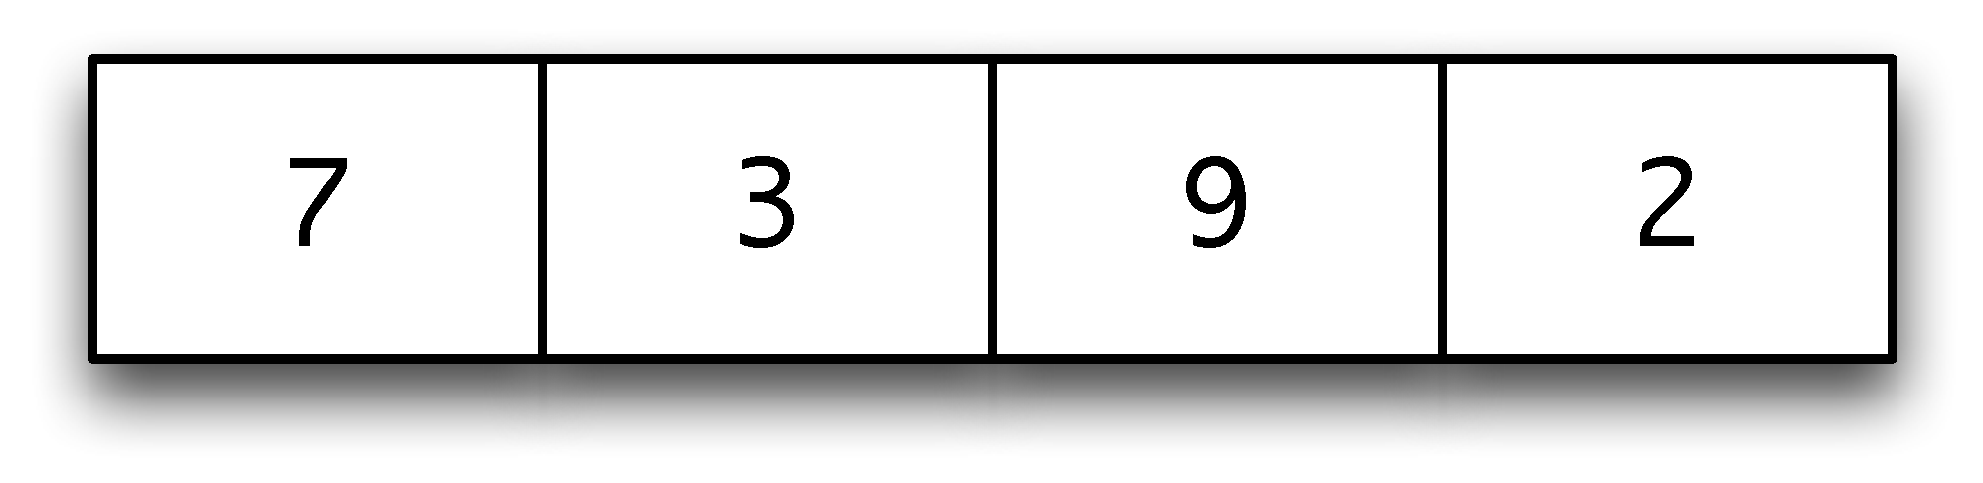
\includegraphics[height=1cm]{Pictures/list1.pdf}\\
is to sort the tail \texttt{[3,9,2]} to give\\
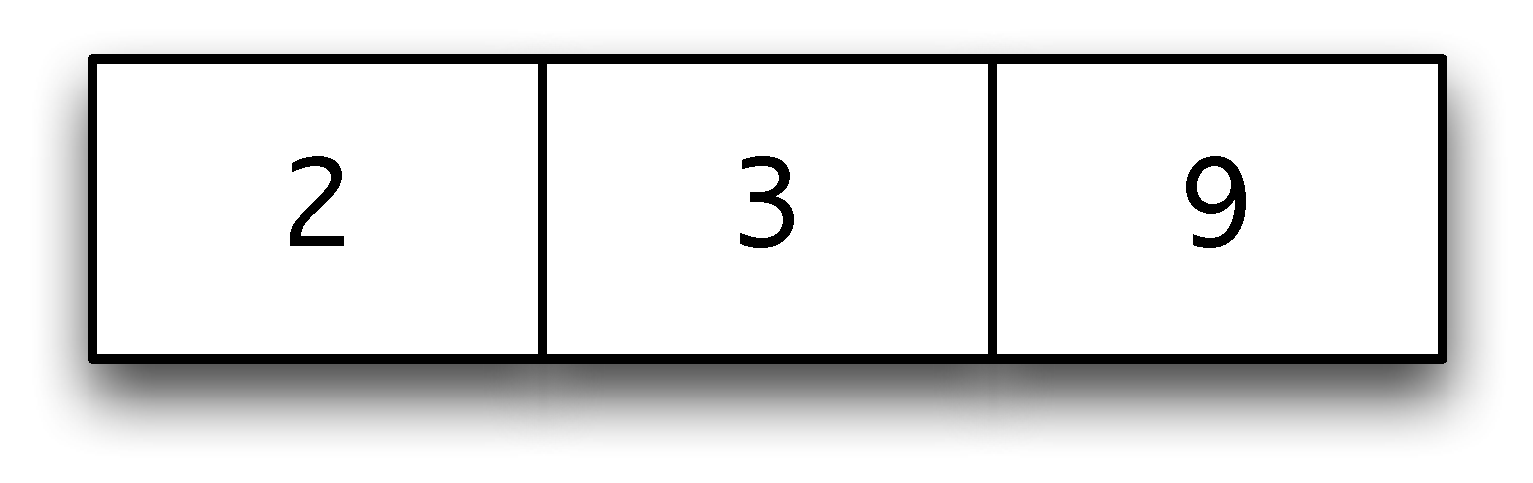
\includegraphics[height=1cm]{Pictures/list2.pdf}\\
It is then a matter of inserting the head, {\mi 7}, in the right place in
this list, to give the result\\
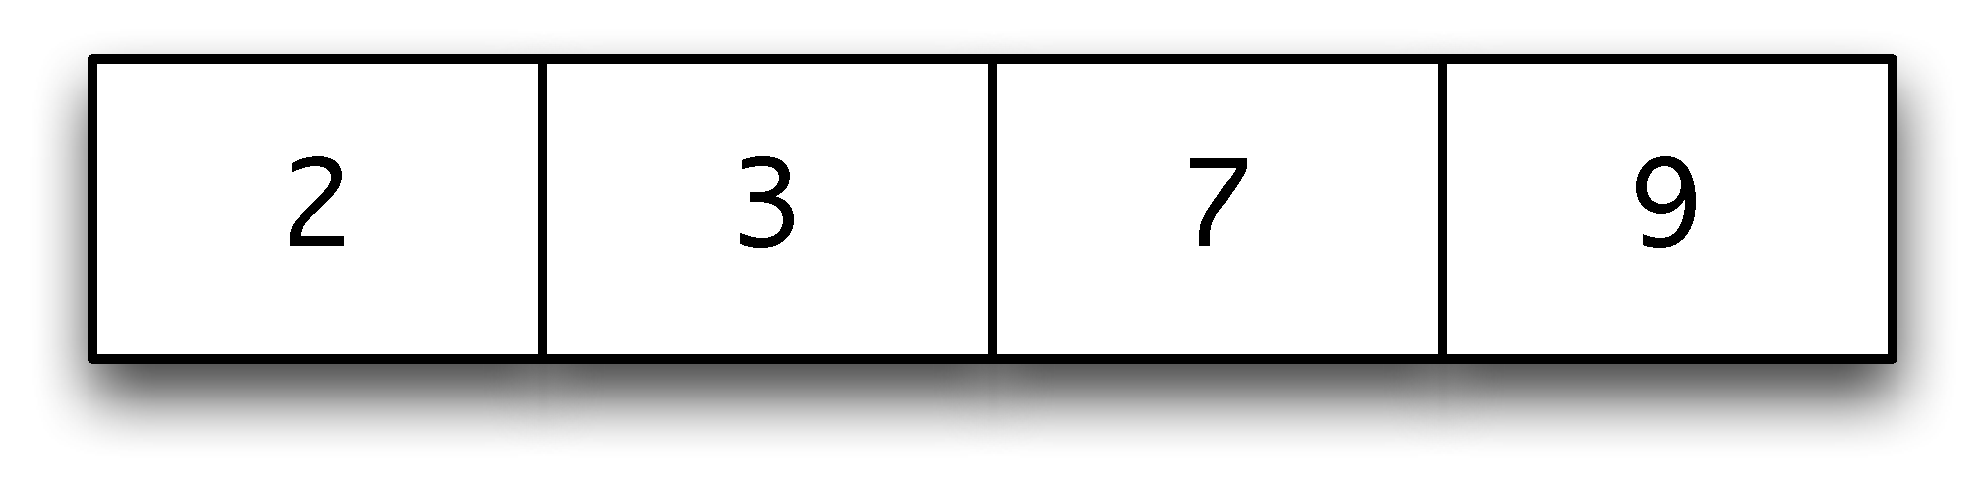
\includegraphics[height=1cm]{Pictures/list3.pdf}\\
This gives the definition of \texttt{iSort} -- the `\texttt{i}' is for
\textbf{ insertion} sort.\index{sorting!insertion}
\begin{alltt}
iSort :: [Integer] -> [Integer]\minx{iSort}
\bl
iSort []     = [] \hfill (iSort.1)
iSort (x:xs) = ins x (iSort xs) \hfill (iSort.2)
\end{alltt}
This is a typical example of top-down\index{design!top-down}
definition, first discussed in Section \ref{designProgram}. We have defined \texttt{iSort}
assuming we can define \texttt{ins}\minx{ins}.
The development of the program has been
in two separate parts, since we have a definition of the function \texttt{iSort}
using a simpler function \texttt{ins}, together with a definition of the
function \texttt{ins} itself. Solving each sub-problem is simpler than
solving the original problem itself.

Now we have to define the function
\begin{alltt}\minx{ins}
ins :: Integer -> [Integer] -> [Integer]
\end{alltt}
To get some guidance about how \texttt{ins} should behave, we look at
some examples. Inserting \texttt{7} into \texttt{[2,3,9]} was given above, while
inserting \texttt{1} into the same list gives\\
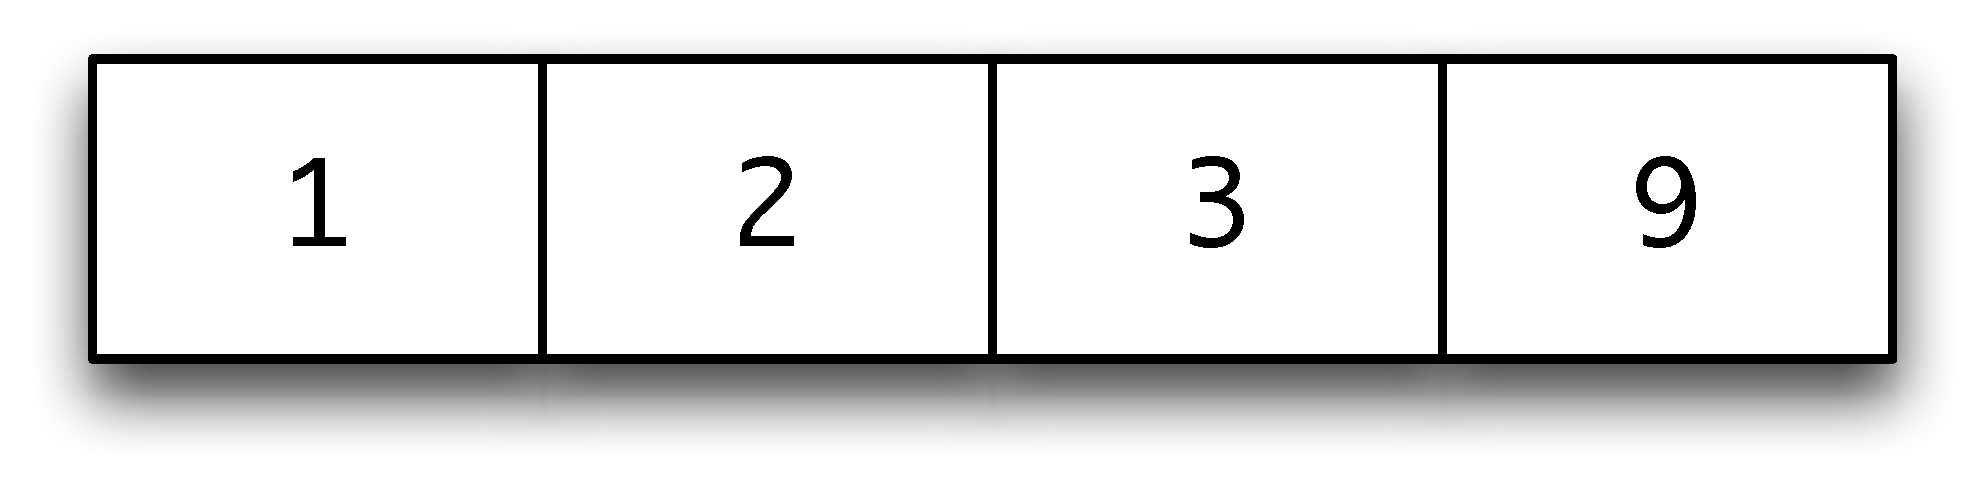
\includegraphics[height=1cm]{Pictures/list4.pdf}\\
Looking at these two examples we see that
\begin{titemize}
\item in the case of \texttt{1}, if the item to be inserted is no larger than
the head of the list, we cons it to the front of the list;
\item In the case of \texttt{7}, if the item is greater than the head, we
insert it in the tail of the list, and cons the head to the result, thus:
\end{titemize}
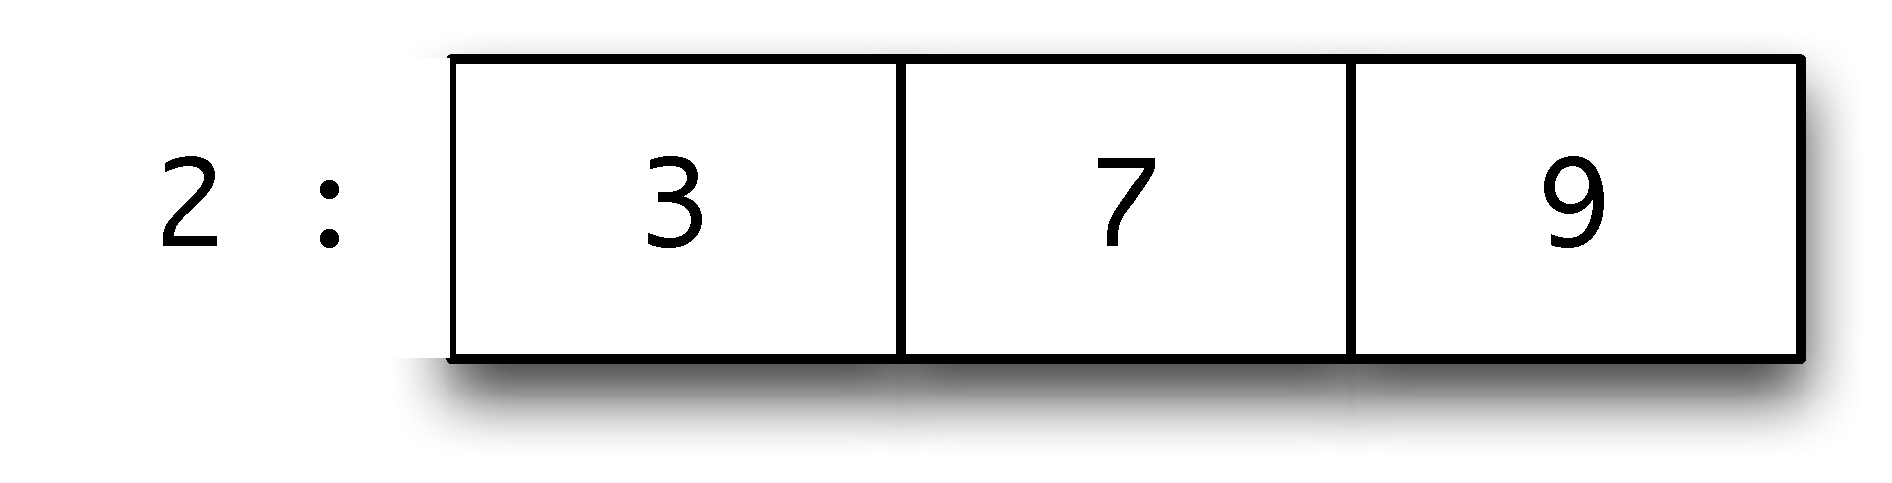
\includegraphics[height=1cm]{Pictures/list5.pdf}\\
The function can now be defined, including the case that the list is empty.
\begin{alltt}
ins x []    = [x] \hfill(ins.1)
ins x (y:ys) 
  | x <= y      = x:(y:ys)\hfill(ins.2)
  | otherwise   = y : ins x ys\hfill(ins.3)
\end{alltt}
We now show the functions in action, in the calculation\index{calculation} 
of \texttt{iSort [3,9,2]}:
\begin{alltt}
iSort [3,9,2]
\step ins 3 (iSort [9,2]) \hfill {\rm by} (iSort.2)
\step ins 3 (ins 9 (iSort [2])) \hfill {\rm by} (iSort.2)
\step ins 3 (ins 9 (ins 2 (iSort []))) \hfill {\rm by} (iSort.2)
\step ins 3 (ins 9 (ins 2 [])) \hfill {\rm by} (iSort.1)
\step ins 3 (ins 9 [2]) \hfill {\rm by} (ins.1)
\step ins 3 (2 : ins 9 []) \hfill {\rm by} (ins.3)
\step ins 3 [2,9] \hfill {\rm by} (ins.1)
\step 2 : ins 3 [9] \hfill {\rm by} (ins.3)
\step 2 : [3,9] \hfill {\rm by} (ins.2)
\step [2,3,9]
\end{alltt}
Developing this function has shown the advantage of looking at examples
while trying to define a function; the examples can give a guide about
how the definition might break into cases, or the pattern of the
recursion. We also saw how using top-down design can break a larger problem
into smaller problems which are easier to solve.

In the next section we look at definitions by more general forms of
recursion.

\index{design!list functions|)}
\index{primitive recursion!list|)}
\index{design!where do I start?|)}
\index{primitive recursion!finding definitions|)}
\end{example}
\begin{exercises}


\item
Test your implementations against the built-in definitions, using the method outlined on page \pageref{qcretest}.


\item Using primitive recursion over lists, define a function
\begin{alltt}
elemNum :: Integer -> [Integer] -> Integer
\end{alltt}
so that \texttt{elemNum x xs} returns the number of times that
\texttt{x} occurs in the list \texttt{xs}. 

Can you define \texttt{elemNum} without using primitive recursion,
using list comprehensions and built-in functions instead?

\item Define a function
\begin{alltt}
unique :: [Integer] -> [Integer]
\end{alltt}
so that \texttt{unique xs} returns the list of elements of \texttt{xs}
which occur exactly once. For example, \texttt{unique [4,2,1,3,2,3]} is
\texttt{[4,1]}. You might like to think of two solutions to this
problem: one using list comprehensions and the other not.

\item 
Can you write a property which links \texttt{elemNum} and \texttt{unique} from the previous two questions? Check to see whether this property does hold using QuickCheck.

\item
Give primitive recursive definitions of the prelude functions
\texttt{reverse} and \texttt{unzip}.


\item Can you use the \texttt{iSort} function to find the minimum and maximum
elements of a list of numbers? How would you find these elements without using
\texttt{iSort}? 

\item
Design test data for the \texttt{ins} function. Your data should address
different possible points of insertion, and also look at any exceptional
cases.

\item
Define a function
\begin{alltt}
isSorted :: [Integer] -> Bool
\end{alltt}
which is true when its argument is sorted in ascending order. How could you use this to write QuickCheck properties to check your \texttt{iSort} and \texttt{ins} functions?

\item {[Harder]}
Is it enough to test that the result of \texttt{iSort} is sorted? What other property should a sorting function have? Can you write a QuickCheck property to check this?


\item
By modifying the definition of the \texttt{ins} function we can change the
behaviour of the sort, \texttt{iSort}. Redefine \texttt{ins} in two different ways
so that 
\begin{titemize}
\item the list is sorted in descending order;
\item duplicates are removed from the list. For example,
\begin{alltt}
iSort [2,1,4,1,2] = [1,2,4]
\end{alltt}
under this definition. 
\end{titemize}

\item
Would you need to redefine your function \texttt{isSorted} to deal with the two different variations of sorting discussed in the last question? If so, how would you modify it; if not, explain why not.

\item
Design test data for the duplicate-removing version of
\texttt{iSort}, explaining your choices.

\item
By modifying the definition of the \texttt{ins} and \texttt{iSort} functions, 
define a function to sort lists of pairs of numbers. The ordering should
be \textbf{lexicographic} -- the dictionary ordering. 
\index{order!lexicographic} This ordering first
looks at the first halves of the pairs; only if these values are equal
are the second halves compared. For instance, \texttt{(2,73)}
is smaller than \texttt{(3,0)}, and this is smaller than \texttt{(3,2)}.
\end{exercises}

\section{General recursions over lists}
\index{general recursion!over lists|(}

Just as we argued in Section \ref{genRecursion}, a recursive definition
of a function need not always use the value of the function
on the tail;  any recursive call to
a value on a {\em simpler\/} list will be legitimate, and so a number of
different patterns of recursion are available for finding function
definitions over lists.
In trying to use recursion over lists to define a function we need to pose the
question:

\subsubsection*{In defining {\tt f (x:xs)} which values
of {\tt f ys} would help me to work out the answer?}

\begin{example}
\subexample*{1.} 
It is possible to use recursion over two arguments simultaneously, 
an example being the definition of the prelude function \texttt{zip}.
Recall that here we turn two lists into a list of pairs,
\begin{alltt}\minx{zip}
zip :: [a] -> [b] -> [(a,b)]
\end{alltt}
with the examples
\begin{alltt}
zip [1,5] ['c','d']     = [(1,'c'), (5,'d')]
zip [1,5] ['c','d','e'] = [(1,'c'), (5,'d')]
\end{alltt}
If each of the lists is non-empty, we form a pair from their heads,
and then zip their tails, giving
\begin{alltt}
zip (x:xs) (y:ys) = (x,y) : zip xs ys\hfill(zip.1)
\end{alltt}
but in all other cases -- that is when at least one of the lists is empty -- 
the result is empty:
\begin{alltt}
zip _ _ = []\hfill(zip.2)
\end{alltt}
Note that we rely on the sequential nature of pattern matching
here;\index{pattern matching!sequentiality of} we can give the patterns
for \texttt{(zip.2)} explicitly if we wish, thus:
\begin{alltt}
zip (x:xs) (y:ys) = (x,y) : zip xs ys
zip (x:xs) []     = []
zip []     zs     = []
\end{alltt}
and in the second definition we see the three separate cases given in
three separate equations. Using the original definition, an example
calculation gives
\begin{alltt}
zip [1,5] ['c','d','e']
\step (1,'c') : zip [5] ['d','e']\hfill\textrm{by }(zip.1)
\step (1,'c') : (5,'d') : zip [] ['e']\hfill\textrm{by }(zip.1)
\step (1,'c') : (5,'d') : []\hfill\textrm{by }(zip.2)
\step (1,'c') : [ (5,'d') ]\hfill\textrm{by defn\ of} :
\step [ (1,'c') , (5,'d') ]\hfill\textrm{by defn\ of} :
\end{alltt}
Note that we have used the fact that `\texttt{:}' is right
associative in writing this calculation.

\subexample*{2.} 
The function \texttt{take} is used to take a given number of values from
a list. For instance, 
\begin{alltt}\minx{take}
take 5  "Hot Rats" = "Hot R"
take 15 "Hot Rats" = "Hot Rats" 
\end{alltt}
In this example we do recursion over an \texttt{Int} and a list
\begin{alltt}
take :: Int -> [a] -> [a]
\end{alltt}
There are some special cases, when the \texttt{Int} is zero, or the list
is empty
\begin{alltt}
take 0 _        = []\hfill(take.1)
take _ []       = []\hfill(take.2)
\end{alltt}
What about the general case, when the list is non-empty and the
\texttt{Int}
greater than zero? We take \texttt{n-1} elements from the tail of the
list, and place the head on the front, thus:
\begin{alltt}
take n (x:xs)
  | n>0         = x : take (n-1) xs\hfill(take.3)
\end{alltt}
and in the other cases we give an error
\begin{alltt}\minx{error}
take _ _        = error "PreludeList.take: negative argument"
\ \hfill(take.4)
\end{alltt}

\subexample*{3.} \index{sorting!quicksort}\index{quicksort}
As a final example, we look at another method for sorting lists (of
integers). The \textbf{quicksort} algorithm works by 
generating {\em two} recursive calls to sort. Suppose we are to sort the
list
\begin{alltt}
                        [4,2,7,1,4,5,6]
\end{alltt}
we can take off the head, \texttt{4}, and then split the result 
\texttt{[2,7,1,4,5,6]} into two parts: 
\begin{alltt}
                        [2,1,4]           [7,5,6]
\end{alltt}
The first contains the elements no larger than \texttt{4}, the
second those exceeding \texttt{4}. We sort these two, giving
\begin{alltt}
                        [1,2,4]           [5,6,7]
\end{alltt}
and then we get an ordered version of the original list thus
\begin{alltt}
                        [1,2,4] ++ [4] ++ [5,6,7]
\end{alltt}
We can write this now
\begin{alltt}
qSort :: [Integer] -> [Integer]

qSort [] = []\hfill(qSort.1)
qSort (x:xs) 
  = qSort [ y | y<-xs , y<=x] ++ [x] ++ qSort [ y | y<-xs , y>x]
\ \hfill(qSort.2)
\end{alltt}
It is striking to see how close this program is to our informal
description of the algorithm, and this expressiveness is one 
of the important advantages of a functional approach.
 
We can see that this recursion will give an answer for every finite
list, since in the recursive calls we apply \texttt{qSort} to two
sublists of \texttt{xs}, which are necessarily smaller than
\texttt{(x:xs)}.


In Chapter \ref{behaviour} we talk about the efficiency of various
algorithms, and show that in general quicksort will be more efficient
than insertion sort.
In the following section we look at a larger example of definitions
which use general forms of recursion.
\end{example}

\begin{exercises}
\item 
Using the definition of \texttt{take} as a guide,
define the prelude functions \texttt{drop} and \texttt{splitAt}. Write QuickCheck tests for these re-defined functions.

\item
What is the value of \texttt{take (-3) []} according to the definition
of \texttt{take} given earlier? How would you modify the definition so
that there is an error reported whenever the \texttt{Int} argument is
negative?


\item
The \texttt{zip} function takes its two arguments separately: we can define this variant to take the arguments as a pair:
\begin{alltt}
zip' :: ([a],[b]) -> [(a,b)]
zip' (xs,ys) = zip xs ys
\end{alltt}
There's a built-in function, which has the reverse effect, taking a list of pairs into a pair of lists:
\begin{alltt}
unzip :: [(a,b)] -> ([a],[b])
\end{alltt}
Write a property for \texttt{zip'} and \texttt{unzip} that expresses that they are the `inverse' of each other: does it matter the order in which they are applied? Try both ways, and see what happens when you apply \texttt{quickCheck} in each case.
 
\item
How would you define a function \texttt{zip3} which zips together three
lists? Try to write a recursive definition and also one which {\em
uses\/} \texttt{zip} instead; what are the advantages and disadvantages
of the two different definitions?

\item
How would you modify \texttt{qSort} to sort a list into descending order?
How would you ensure that \texttt{qSort} removed duplicate elements?

\item
One list is a \textbf{sublist} of another if the elements of the first occur in the
second, in the same order. For instance, \texttt{"ship"} is a sublist
of \texttt{"Fish \& Chips"}, but not of \texttt{"hippies"}.

A list is a \textbf{subsequence} of another if it occurs as a sequence
of elements {\em next to each other}. For example, \texttt{"Chip"} is a
subsequence
of \texttt{"Fish \& Chips"}, but not of \texttt{"Chin up"}.

Define functions which decide whether one string is a sublist or a
subsequence of another string.

\item
Write QuickCheck properties which test your implementations of the tests for `sublist' and `subsequence'.

\end{exercises}

\section{Example: text processing}
\index{examples!text processing|see{text processing}}
\index{text processing|(}
\label{textProc}

In word processing systems it is customary for lines to be filled and
broken automatically, to enhance the appearance of the
text. This book is no exception. Input of the form
\begin{alltt}
{\hskip1pc}The heat bloomed     in December
 as the   carnival  season
            kicked into  gear.
Nearly helpless with sun and glare, I avoided Rio's brilliant
sidewalks
  and glittering beaches,
panting in dark   corners
and waiting out the inverted southern summer.
\end{alltt}
would be transformed by \textbf{filling} to \index{text processing!filling}
\begin{alltt}
{\hskip1pc}The heat bloomed in December as the
carnival season kicked into gear.
Nearly helpless with sun and glare,
I avoided Rio's brilliant sidewalks
and glittering beaches, panting in
dark corners and waiting out the
inverted southern summer.
\end{alltt}
To align the right-hand margin, the text is \textbf{justified} by adding extra
\index{text processing!justification}
inter-word spaces on all lines but the last:
\begin{alltt}
{\hskip1pc}The heat bloomed in December as the
carnival  season  kicked into gear.
Nearly helpless with sun and glare,
I avoided Rio's brilliant sidewalks
and glittering beaches, panting  in
dark  corners  and  waiting out the
inverted southern summer.
\end{alltt}
An input file in Haskell can be
treated as a string of characters, and so string-manipulating operations
play an important role here. Also, since strings are lists, this example
will exercise general list functions.

\subsection*{Overall strategy}

In this section we give an example of bottom-up program development,
thinking first about some of the components we will need to solve the
problem, rather than decomposing the solution in a top-down way.
\index{design!bottom up}

The first step in processing text will be to split an input string into 
\textbf{words}, discarding any white space. The words are then rearranged into
lines of the required length. These lines can then have spaces added so as to
justify the text. We therefore start by looking at how text is split into
\index{text processing!splitting into words}
words. 

\subsection*{Extracting words}

We first ask, given a string of characters, how should we define a
function to take the first word from the front of a string? 

A word is any sequence which does not contain
the \textbf{whitespace} characters space, tab and newline. 
\begin{alltt}
whitespace = ['\bs{n}','\bs{t}',' ']\minx{whitespace}
\end{alltt}
In defining \texttt{getWord} we will use the standard function \texttt{elem},
which tests whether an object is an element of a list. For instance,  
\texttt{elem 'a' whitespace} is \texttt{False}.

To guide the
definition, consider two examples.
\begin{itemize}
\item \texttt{getWord " boo"} should be \texttt{""} as the first character is
whitespace;
\item \texttt{getWord "cat dog"} is \texttt{"cat"}. We get this by putting {\mi
'c'} on the front of \texttt{"at"}, which is \texttt{getWord "at dog"}.
\end{itemize}
The definition is therefore given by:
\begin{alltt}
getWord :: String -> String\minx{getWord}
getWord []    = [] \hfill (getWord.1)
getWord (x:xs) 
  | elem x whitespace   = []\hfill(getWord.2)
  | otherwise           = x : getWord xs\hfill (getWord.3)
\end{alltt}
Consider an example
\begin{alltt}
getWord "cat dog"
\step 'c' : getWord "at dog" \hfill {\rm by} (getWord.3)
\step 'c' : 'a' : getWord "t dog" \hfill {\rm by} (getWord.3)
\step 'c' : 'a' : 't' : getWord " dog" \hfill {\rm by} (getWord.3)
\step 'c' : 'a' : 't' : [] \hfill {\rm by} (getWord.2)
\step "cat"
\end{alltt}
In a similar way, the first word of a string can be dropped.
\begin{alltt}
dropWord :: String -> String\minx{dropWord}
dropWord []    = []
dropWord (x:xs) 
  | elem x whitespace   = (x:xs)
  | otherwise           = dropWord xs
\end{alltt}
It is easy to check that \texttt{dropWord "cat dog" = " dog"}. We aim to
use the functions \texttt{getWord} and \texttt{dropWord} to split a string
into its constituent words. Note that before we take a word from the
string \texttt{" dog"}, we should remove the whitespace character(s) from the
front. The function \texttt{dropSpace} will do this.
\begin{alltt}
dropSpace :: String -> String\minx{dropSpace}
dropSpace []    = []
dropSpace (x:xs) 
  | elem x whitespace   = dropSpace xs
  | otherwise           = (x:xs)
\end{alltt}
How is a string \texttt{st} to be split into words? Assuming \texttt{st} has no
whitespace at the start,
\begin{titemize}
\item the first word in the output will be given by applying \texttt{getWord} to
\texttt{st};
\item the remainder will be given by splitting what remains after removing
the first word and the space following it:
\texttt{dropSpace (dropWord st)}.
\end{titemize}
The top-level function \texttt{splitWords} calls \texttt{split} after removing any
whitespace at the start of the string. 
\begin{alltt}
type Word = String\minx{Word}
\bl
splitWords :: String -> [Word]\minx{splitWords}
splitWords st = split (dropSpace st)
\bl
split :: String -> [Word]
split [] = []
split st
  = (getWord st) : split (dropSpace (dropWord st))
\end{alltt}
Consider a short example.
\begin{alltt}
splitWords "  dog cat"
\step split "dog cat"
\step (getWord "dog cat")
         : split (dropSpace (dropWord "dog cat"))
\step "dog" : split (dropSpace " cat")
\step "dog" : split "cat"
\step "dog" : (getWord "cat")
         : split (dropSpace (dropWord "cat"))
\step "dog" : "cat" : split (dropSpace [])
\step "dog" : "cat" : split []
\step "dog" : "cat" : []
\step [ "dog" , "cat" ]
\end{alltt}

\subsection*{Splitting into lines}

Now we have to consider how to break a list of words into lines. As before,
we look to see how we can take the first line from a list of words. 
\begin{alltt}
type Line = [Word]
getLine :: Int -> [Word] -> Line\minx{getLine}
\end{alltt}
\texttt{getLine} takes two parameters. The first is the length of the line to be
formed, and the second the list from which the words are taken. The definition 
uses \texttt{length} to give the length of a list.
The definition will have three cases
\begin{titemize}
\item In the case that no words are available, the line formed is empty.
\item If the first word available is \texttt{w}, then this goes on the line if
there is room for it: its length, \texttt{length w}, has to be no greater than the
length of the line, \texttt{len}.\\
 The remainder of the line is built from the 
words that remain by taking a
line of length  \texttt{len-(length w+1)}.
\item If the first word does not fit, the line has to be empty. 
\end{titemize}
\begin{alltt}
getLine len []     = []
getLine len (w:ws)
  | length w <= len     = w : restOfLine  
  | otherwise           = []
    where
    newlen      = len - (length w + 1)
    restOfLine  = getLine newlen ws
\end{alltt}
Why is the \texttt{rest} of the line of length \texttt{len-(length w+1)}? Space must
be allocated for the word \texttt{w} {\em and\/} the inter-word space needed to separate
it from the word which follows. How does the function work in an example?
\begin{alltt}
getLine 20 ["Mary","Poppins","looks","like",...
\step "Mary" : getLine 15 ["Poppins","looks","like",...
\step "Mary" : "Poppins" : getLine 7 ["looks","like",...
\step "Mary" : "Poppins" : "looks" : getLine 1 ["like",...
\step "Mary" : "Poppins" : "looks" : []
\step [ "Mary" , "Poppins" , "looks" ]
\end{alltt}
A companion function,
\begin{alltt}
dropLine :: Int -> [Word] -> Line\minx{dropLine}
\end{alltt}
removes a line from the front of a list of words, just as \texttt{dropWord} is a
companion to \texttt{getWord}. The function to split a list of words
into lines of length at most (the constant value) \texttt{lineLen} can now be defined:
\begin{alltt}
splitLines :: [Word] -> [Line]\minx{splitLines}
splitLines [] = []
splitLines ws
  = getLine lineLen ws
         : splitLines (dropLine lineLen ws)
\end{alltt}
This concludes the definition of the function \texttt{splitLines}, which gives
filled lines from a list of words. 

\subsection*{Conclusion}

To fill a text string
into lines, we write
\begin{alltt}
fill :: String -> [Line]\minx{fill}
fill = splitLines . splitWords
\end{alltt}
To make the result into a single string we need to write a function 
\begin{alltt}
joinLines :: [Line] -> String\minx{joinLines}
\end{alltt}
This is left as an exercise, as is justification of lines.
\index{text processing|)}


\begin{exercises}

\item
Define the function \texttt{dropLine}
specified in the text.

\item
Give a definition of the function
\begin{alltt}
{\hskip1pc}joinLine :: Line -> String
\end{alltt}
which turns a line into printable form. For example,
\begin{alltt}
{\hskip1pc}joinLine [ "dog" , "cat" ] = "dog cat"
\end{alltt}

\item
Using the function \texttt{joinLine}, or otherwise, define the function
\begin{alltt}
{\hskip1pc}joinLines :: [Line] -> String
\end{alltt}
which joins together the lines, separated by newlines.

\item
In this case study we have defined separate `take' and `drop' functions for
words and lines.
Redesign the program so that it uses `split' functions -- like the prelude
function \texttt{splitAt} -- instead.

\item
{[Harder]} Modify the function \texttt{joinLine} so that it justifies the
line to length \texttt{lineLen} by adding the appropriate number of spaces
between the words. 

\item
Design a function
\begin{alltt}
{\hskip1pc}wc :: String -> (Int,Int,Int)
\end{alltt}
which when given a text string returns the number of characters, words and
lines in the string. The end of a line in the string is signalled by the
newline character, \texttt{'\bs{n}'}. Define a similar function
\begin{alltt}
{\hskip1pc}wcFormat :: String -> (Int,Int,Int)
\end{alltt}
which returns the same statistics for the text {\em after\/} it has been
filled.

\item
Define a function
\begin{alltt}
{\hskip1pc}isPalin :: String -> Bool
\end{alltt}
which tests whether a string is a palindrome -- that is whether it is the
same read both backwards and forwards. An example is the string
\begin{alltt}
{\hskip1pc}Madam I'm Adam
\end{alltt}
Note that punctuation and white space are ignored in the test, and that no
distinction is made between capital and small letters. You might first like to
develop a test which simply tests whether the string is exactly the same
backwards and forwards, and only afterwards take account of punctuation and
capital letters.

\item
{[Harder]} Design a function
\begin{alltt}
{\hskip1pc}subst :: String -> String -> String -> String
\end{alltt}
so that
\begin{alltt}
subst oldSub newSub st
\end{alltt}
 is the result of replacing the first
occurrence in \texttt{st} of the substring \texttt{oldSub} by the substring \texttt{newSub}. For instance,
\begin{alltt}
{\hskip1pc}subst "much  " "tall " "How much  is that?"
  = "How tall is that?"
\end{alltt}
If the substring \texttt{oldSub} does not occur in \texttt{st}, the result should
be \texttt{st}.

\item {[Harder]} 
Define QuickCheck properties which test the behaviour of your \texttt{subst} function, defined in the previous question.


\index{lists!defining functions|)}
\index{general recursion!over lists|)}
\end{exercises}



\begin{summary}
This chapter has shown how functions can be defined by recursion over lists, and 
completes our account of the different ways that list-processing functions can be defined.
In the chapter we have looked at examples of the design
principles which we first discussed in Chapter \ref{writingProgs},
including `divide and conquer' and general pieces of advice about
designing recursive programs. The text processing case study provides a
broadly bottom-up approach to defining a library of functions. 
\end{summary}

%\end{document}
